
\documentclass[journal]{IEEEtran}
\usepackage{amsmath}
\usepackage{graphicx}
\usepackage{makecell}
\usepackage{verbatim}
\usepackage[backref]{hyperref}

% 为了避免特定单词的错误连字
\hyphenation{op-tical net-works semi-conduc-tor}


\begin{document}
\title{Energy Efficiency Fast Fourier Transform Design \\ Based on Computing-in-Memory}
\author{Run Liu, \IEEEmembership{Student Member, IEEE,}
        Kejie Huang, \IEEEmembership{Senior Member, IEEE}}

\maketitle
\begin{abstract}
Fast Fourier Transform(FFT) is a widely used algorithm in digital signal processing while it costs a lot of energy and storages. Computing-In-Memory(CIM) is an emerging technology which can realize computation and storage in same memory cell. This brief explores and analyzes the FFT design combine with CIM technology for energy efficiency improvement. In order to flexibly apply different points FFT to different CIM array, we using Mixed-Radix FFT method to decompose the big twiddle factor matrix to several small ones. The simulation results show that our proposed 8-bit 512 points FFT-CIM design only costs 21.66mW.
\end{abstract}

\begin{IEEEkeywords}
CIM, FFT, Mix-Radix, Energy Efficiency.
\end{IEEEkeywords}


\section{Introduction}
\IEEEPARstart{F}{FT} is an essential algorithm which convert signal from time domain into frequency domain, it can be used in many fields such as mathematics, physics, engineering, artificial intelligence, etc. In the age of Internet of Things(IoT), we have many ultra-low-power devices such as cell phone, wireless sensor nodes and implantable biomedical devices \cite{1}. In the same time, FFT is a high throughput application which will costs a lot of energy in computing. There is a dilemma which is developing FFT application scenarios in ultra-low-power devices while FFT needs high energy consumption. However, the emerging CIM technology is a good choice to solve above issues. In the traditional Von-Neumann computing architecture, the memory module and the computing module are separated, which will cause serious\cite{2} "memory wall" effect with the speed dismatch between memory and Central Processing Unit(CPU). The existence of the well-known 'memory-bottleneck' inherent in the state-of-art Von-Neumann computing model poses a major constrain for energy efficient and high throughput computations. Computing-in-Memory technology is a technology that uses novel memory devices to realize storage and computing function at the same place. The chip architecture based on CIM technology not only realizes the identity of storage and computing, eliminates the "memory wall" effect, and reduces power consumption, but also its multiplication and accumulation computing mode is very suitable for modern AI model represented by convolutional neural network. The calculation and treatment of power system.

Recently, the research of FFT mainly focuses on using various methods to improve the computing speed and reduce the hardware cost. For example, the single port memory is used to merge the memory into four memories and perform arbitrary radix-2 FFT calculation, so that the input and output can run with the same parallelism as the internal processing to improve the throughput; or the capacitor is used as the memory unit to design the asynchronous random adder to improve the area of FFT design; and the low rank tensor approximation is also used to simplify the FFT calculation process; at the same time, tensor decomposition is used to store rotation factor matrix to reduce memory consumption. The FFT computation is optimized by methods such as tensor decomposition and adjustment of in memory structure, but there is not much research on the optimization of FFT computation by using new in memory computing technology\cite{12,13}.

FFT is suitable for a large number of computation. For the key word spotting application, which can use both feature extraction and neural network convolution by computing in memory technology, it is predictable to reduce the power consumption, which is also an important direction of keyword detection design optimization. At the same time, for other neural network models, which convert data from the original domain to the frequency domain, using computing in memory technology to optimize the conversion mode is also a feasible method of hardware optimization.

In this paper, we propose a energy efficiency design based on CIM architecture. We make the following key contributions compared to other designs:


%\subsection{Subsection Heading Here}
%Subsection text here.

% needed in second column of first page if using \IEEEpubid
%\IEEEpubidadjcol

\subsubsection{Analyse the feasibility of combining FFT and CIM}
The essence of CIM computation is multiplication and accumulation, while
we will do many matrix calculation in FFT. Matrix calculation is also multiplication and accumulation in essence. We can combine both of them to design FFT-CIM.
\subsubsection{Implementation of FFT based on Mix-Radix decomposition}
Because of the large matrix of rotation factor in the traditional DFT matrix calculation mode, it is difficult to calculate the matrix directly by in memory calculation without considering the corresponding optimization of DFT. The mixed radix decomposition method based on FFT can transform a single large rotation factor matrix  into multiple small matrices, which can realize practical FFT design in CIM module.
\subsubsection{Analyse the different Mix-Radix decomposition metrics of design}
For different application scenarios, we may need different points of FFT. For example, in the field of speech recognition, the commonly used number of FFT points is 512. Therefore, we analyze the resource consumption and performance of different FFT points (N = 512/1024/2048) under different mixed radix decomposition methods.

The rest of paper is organized as follows. In section II, we elaborate the background of CIM and Mix-Radix
decomposition method. The overall architecture of FFT-CIM is proposed in section III. In section IV, we
implement different FFT in different mix-radix decomposition\cite{8,9,10,11}method and show the experiment result. Finally, we make a brief conclusion in section V.

\section{Background}
\subsection{Background of Computing-in-Memory Technology}
Computing in memory is a new type of computing mode. The integration of storage and computing units is the main feature of this technology, which means that the transportation of data from other memory units to computing units can be saved, so as to reduce a lot of power consumption. The calculation mode of computing in memory is to get the integration of current through the memory cell. This calculation mode is actually a multiplication and accumulation of data, so as to the core calculation of recent AI model, which is the multiplication and accumulation of tensor. We can see many computing in memory cell include SRAM, RRAM, flash and so on. In the same times, there have many computing in memory architecture like a transformer and a resistor, which is 1R1T. This paper also adopts this design structure. With the rapid increase of the amount of data and computation in the AI world, computing in memory technology is developing rapidly. It is widely used not only in the field of AI, but also in the field of traditional database and service center\cite{14}.
\subsection{Background of Mix-Radix Decomposition FFT}
There are many applications will use large number of FFT, the problem is
that will be very inconvenient to use large matrix multiplication, especially for the computing in memory technology. However, a large rotation factor matrix can be decomposed into several small rotation factor matrices in the form of mixed radix, which can be implemented in the computing in memory module friendly. For N-point DFT, if n is a composite number, it can be graded as the product of some factors, then the general algorithm of FFT can be used, that is, the mix radix FFT algorithm, and the commonly used radix-2 algorithm is a special case of this general algorithm.

If $N$ can be expressed as composite number, which is $N=r_1r_2...r_L$, for any integer if $n<r_1r_2...r_L$, we can
expressed this number according to $L$-base $r_1$, $r_2$,..., $r_L$ in the form of multi base and multi system, like $(n_{L-1}n_{L-2}...n_{1}n_{0})_{r_1r_2...r_L}$. The value represented by this multiple base multiple
system is:
\begin{equation}
    (n)_{10} = n_{L-1}(r_2r_3...r_L) +
             n_{L-2}(r_3r_4...r_L) +
             ... +
             n_1n_L +
             n_0
\end{equation}
At the same times, we can get the reverse order number
$[p(n)]_{r_1r_2...r_{L}} = (n_0n_1...n_{L-2}n_{L-1})_{r_Lr_{L-1}...r_1}$, which represents the following values:
\begin{equation}
    [p(n)]_{10} = n_0(r_1r_2...r_{L-1}) +
                  n_1(r_1r_2...r_{L-2}) +
                  ... +
                  n_{L-2}r_1 +
                  n_{L-1}
\end{equation}
In this representation of multi base and multi system:
\begin{equation}
\begin{aligned}
  n_0 &: 0, 1, ..., r_L-1 \\
  n_1 &: 0, 1, ..., r_{L-1}-1 \\
  ... \\
  n_{L-1} &: 0, 1, ..., r_1-1
\end{aligned}
\end{equation}
For example, if we want to decomposition 512 points FFT into three stages, and the decomposed states
is $N=16*16*2$, which means $r_1=16, r_2=16, r_3=2, L=3$, so we will have:
\begin{equation}
    n = n_2(r_2r_3) + n_1r_3 + n_0 = 32n_2 + 2n_1 + n_0
\end{equation}
\begin{equation}
    k = k_0(r_1r_2) + k_1r_1 + k_2 = 256k_0 + 16k_1 + k_2
\end{equation}
\begin{equation}
\begin{aligned}
  n_0,k_0 &: 0 \sim 1 (r_3) \\
  n_1,k_1 &: 0 \sim 15 (r_2) \\
  n_2,k_2 &: 0 \sim 15 (r_1)
\end{aligned}
\end{equation}
We all know that the formula of DFT is $X(k) = \sum\limits_{n=0}^{511}x(n)W_{512}^{nk}$,
if we bring formula(5)-(6) into this DFT formula, we will get the formula of different stages.
\begin{equation}
\begin{aligned}
    X_1(k_2,n_1,n_0) &= \sum_{n_2=0}^{15} x(n_2,n_1,n_0)W_{16}^{n_2k_2} \\
    X_1^{'}(k_2,n_1,n_0) &= X_1(k_2,n_1,n_0) W_{512}^{(2n_1 + n_0)k_2}
\end{aligned}
\end{equation}
\begin{equation}
\begin{aligned}
    X_2(k_2,k_1,n_0) &= \sum_{n_1=0}^{15} X_1^{'}(k_2,n_1,n_0) W_{16}^{n_1k_1} \\
    X_2^{'}(k_2,k_1,n_0) &= X_2(k_2,k_1,n_0) W_{512}^{16n_0k_1}
\end{aligned}
\end{equation}
\begin{equation}
    X(k_2,k_1,k_0) = \sum_{n_0=0}^{1} X_2^{'}(k_2,k_1,n_0) W_{2}^{n_0k_0}
\end{equation}


\section{Design Architecture}
\subsection{Architecture of Design}
Fig.1 shows the overall architecture of the proposed FFT-CIM design. The whole design includes the array of unit DFT module after decomposition. Each unit DFT module is the core of computing in memory array. In the computing in memory array, the rotation factor in FFT will stored in this memory first, including its real part and imaginary part. This calculation array is the core of FFT-CIM design. The external memory unit will stores the original FFT data, and then this data will enter computing in memory array to complete the calculation of each level through certain data selection rules. At the same time, the memory module will also store the intermediate data generated by each stage of computation, which is the result data generated by each stage of computation. In the array of computing in memory, the data generated by each stage is analog. The analog data will convert to digital data through the ADC array shown in the fig.1, that is the results of each stage.

\begin{figure}[h]
\centering
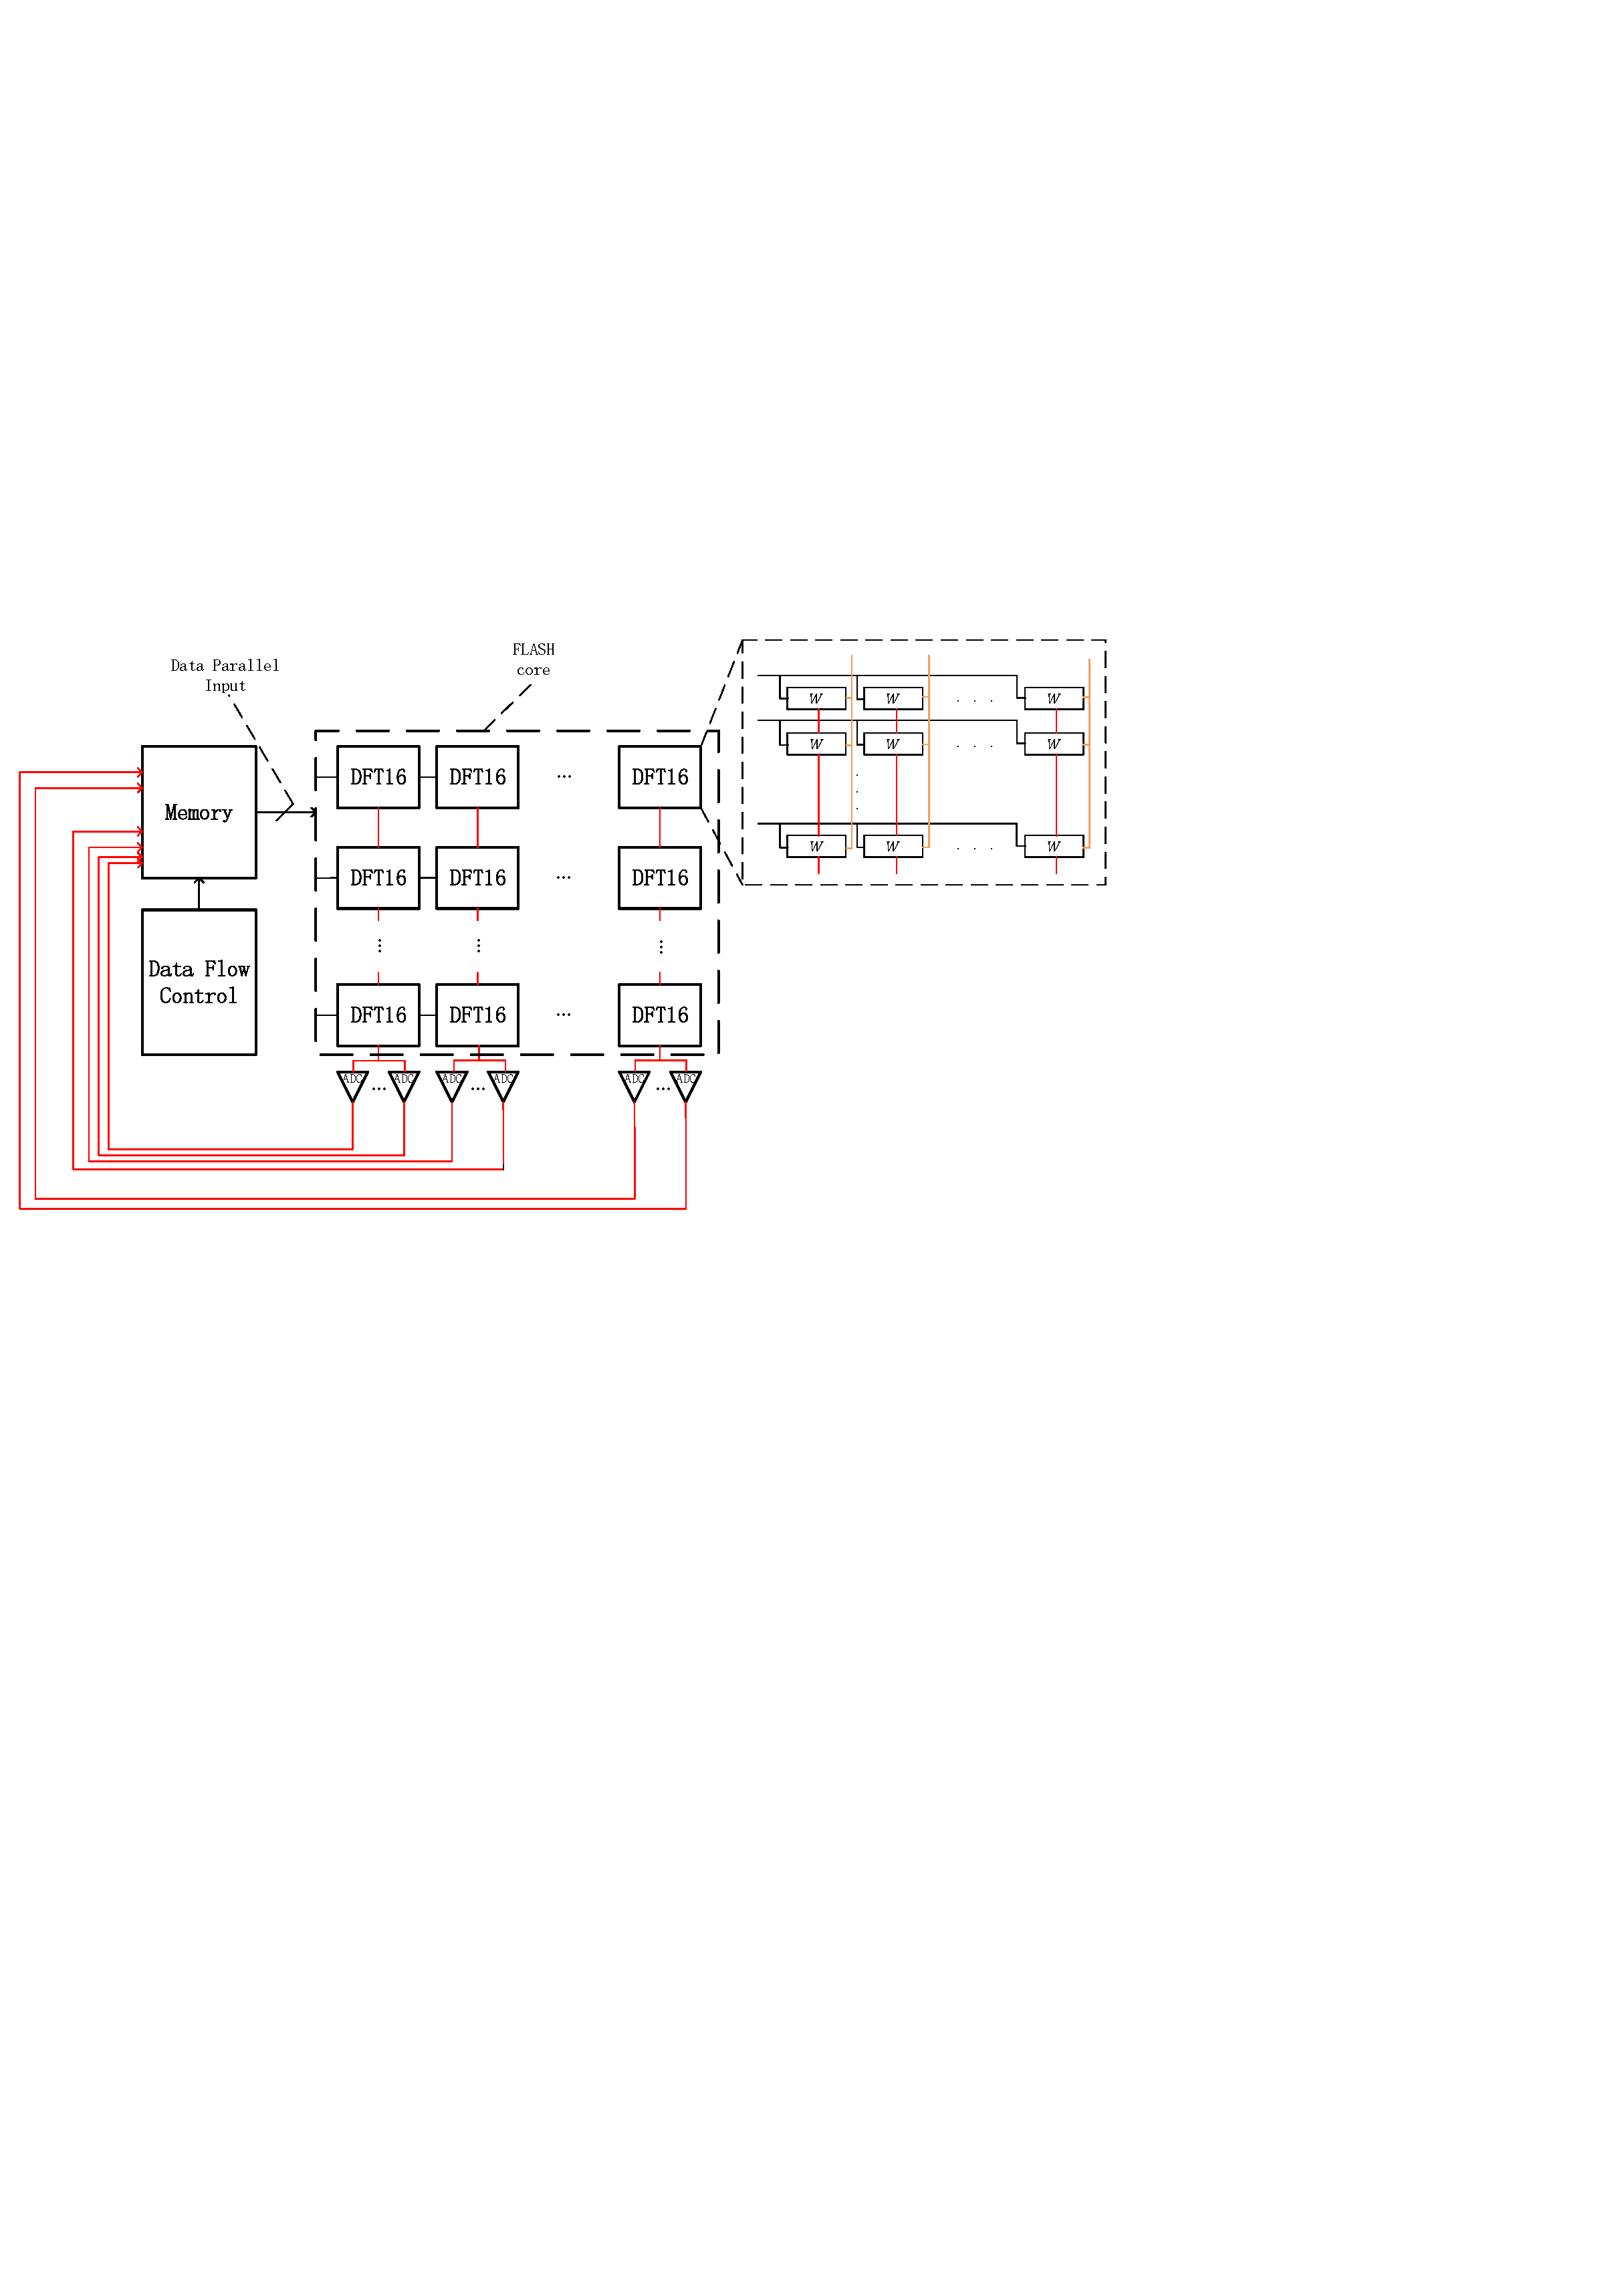
\includegraphics[scale=0.3]{figures/figure1}
\caption{The architecture of the proposed FFT-CIM design}
\end{figure}

In the fig.1, the address generation module is a significant module, which selects data of different addresses to enter the computing in memory module array. In the second chapter of this paper, we see that due to the design of hybrid radix, the sequence order of FFT data input is broken, and each stage needs to select different positions of data for calculation.This means that we need a flexible controller to control the data flow into the computing core, which will be discussed in the following sections.

\subsection{Unit Computing Core}
In Fig.1, we see the overall architecture, in which the core part is the computing in memory unit. Fig.2 is a schematic diagram of a DFT16 module to generate one data. Because of computing in memory is more friendly to matrix multiplication and accumulation, DFT is suitable for CIM array. Its multiply 16 input data and 16 rotation factor data stored in in memory unit to get a result. In the in memory unit, the rotation factor is divided into real part and imaginary part, which are stored separately, and all are calculated with 8 bit data,The computation results of each column will be converted by ADC, and then the digital results will be stored in the storage unit.
\begin{figure}[h]
\centering
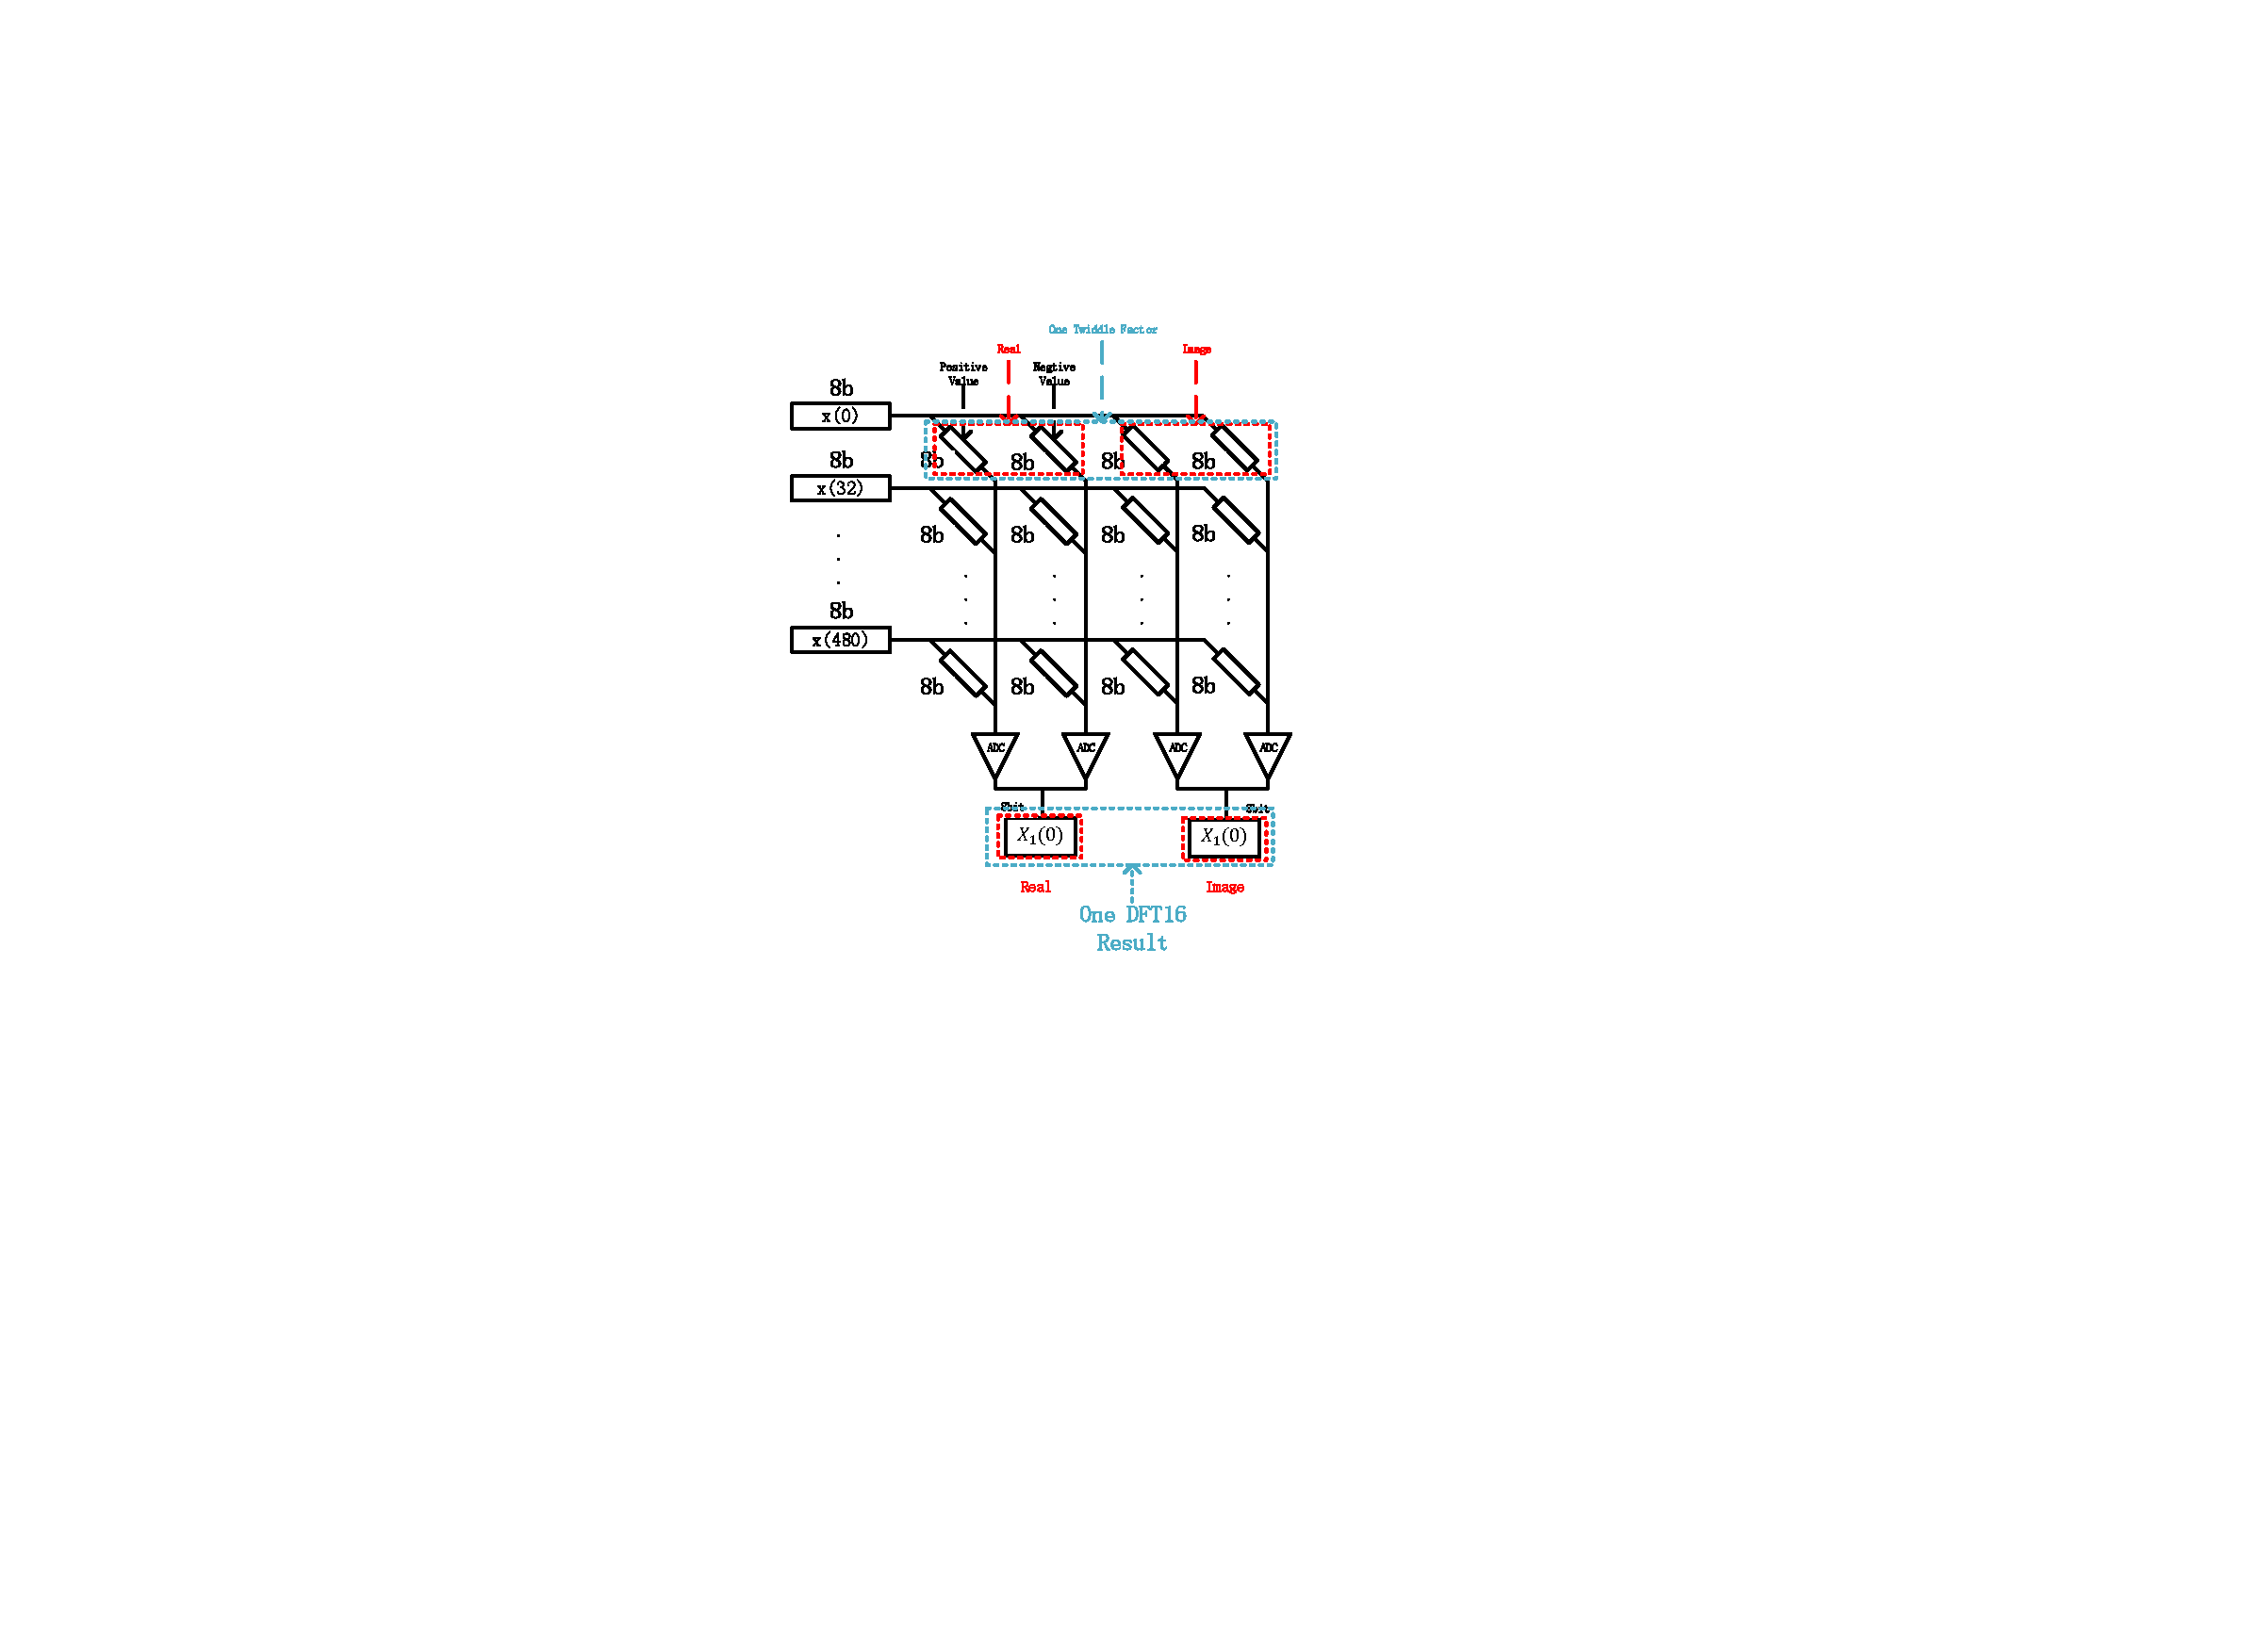
\includegraphics[scale=0.8]{figures/figure2}
\caption{The Computation in CIM}
\end{figure}

Therefore, in the DFT16 module, we arrange the in memory array in Fig.2 horizontally and repeatedly, and store different rotation factor data in the in memory cells of each column, so that we can complete the calculation module of a DFT16 module. In such module, 16 data are input in parallel. After the current integration in the memory unit and ADC conversion, 16 data will be output at the same time. In this way, a computation of DFT16 is completed.

In Fig.3, we show the calculation module of a DFT16 unit. The whole computing in memory array is composed by such modules.

\begin{figure}[h]
\centering
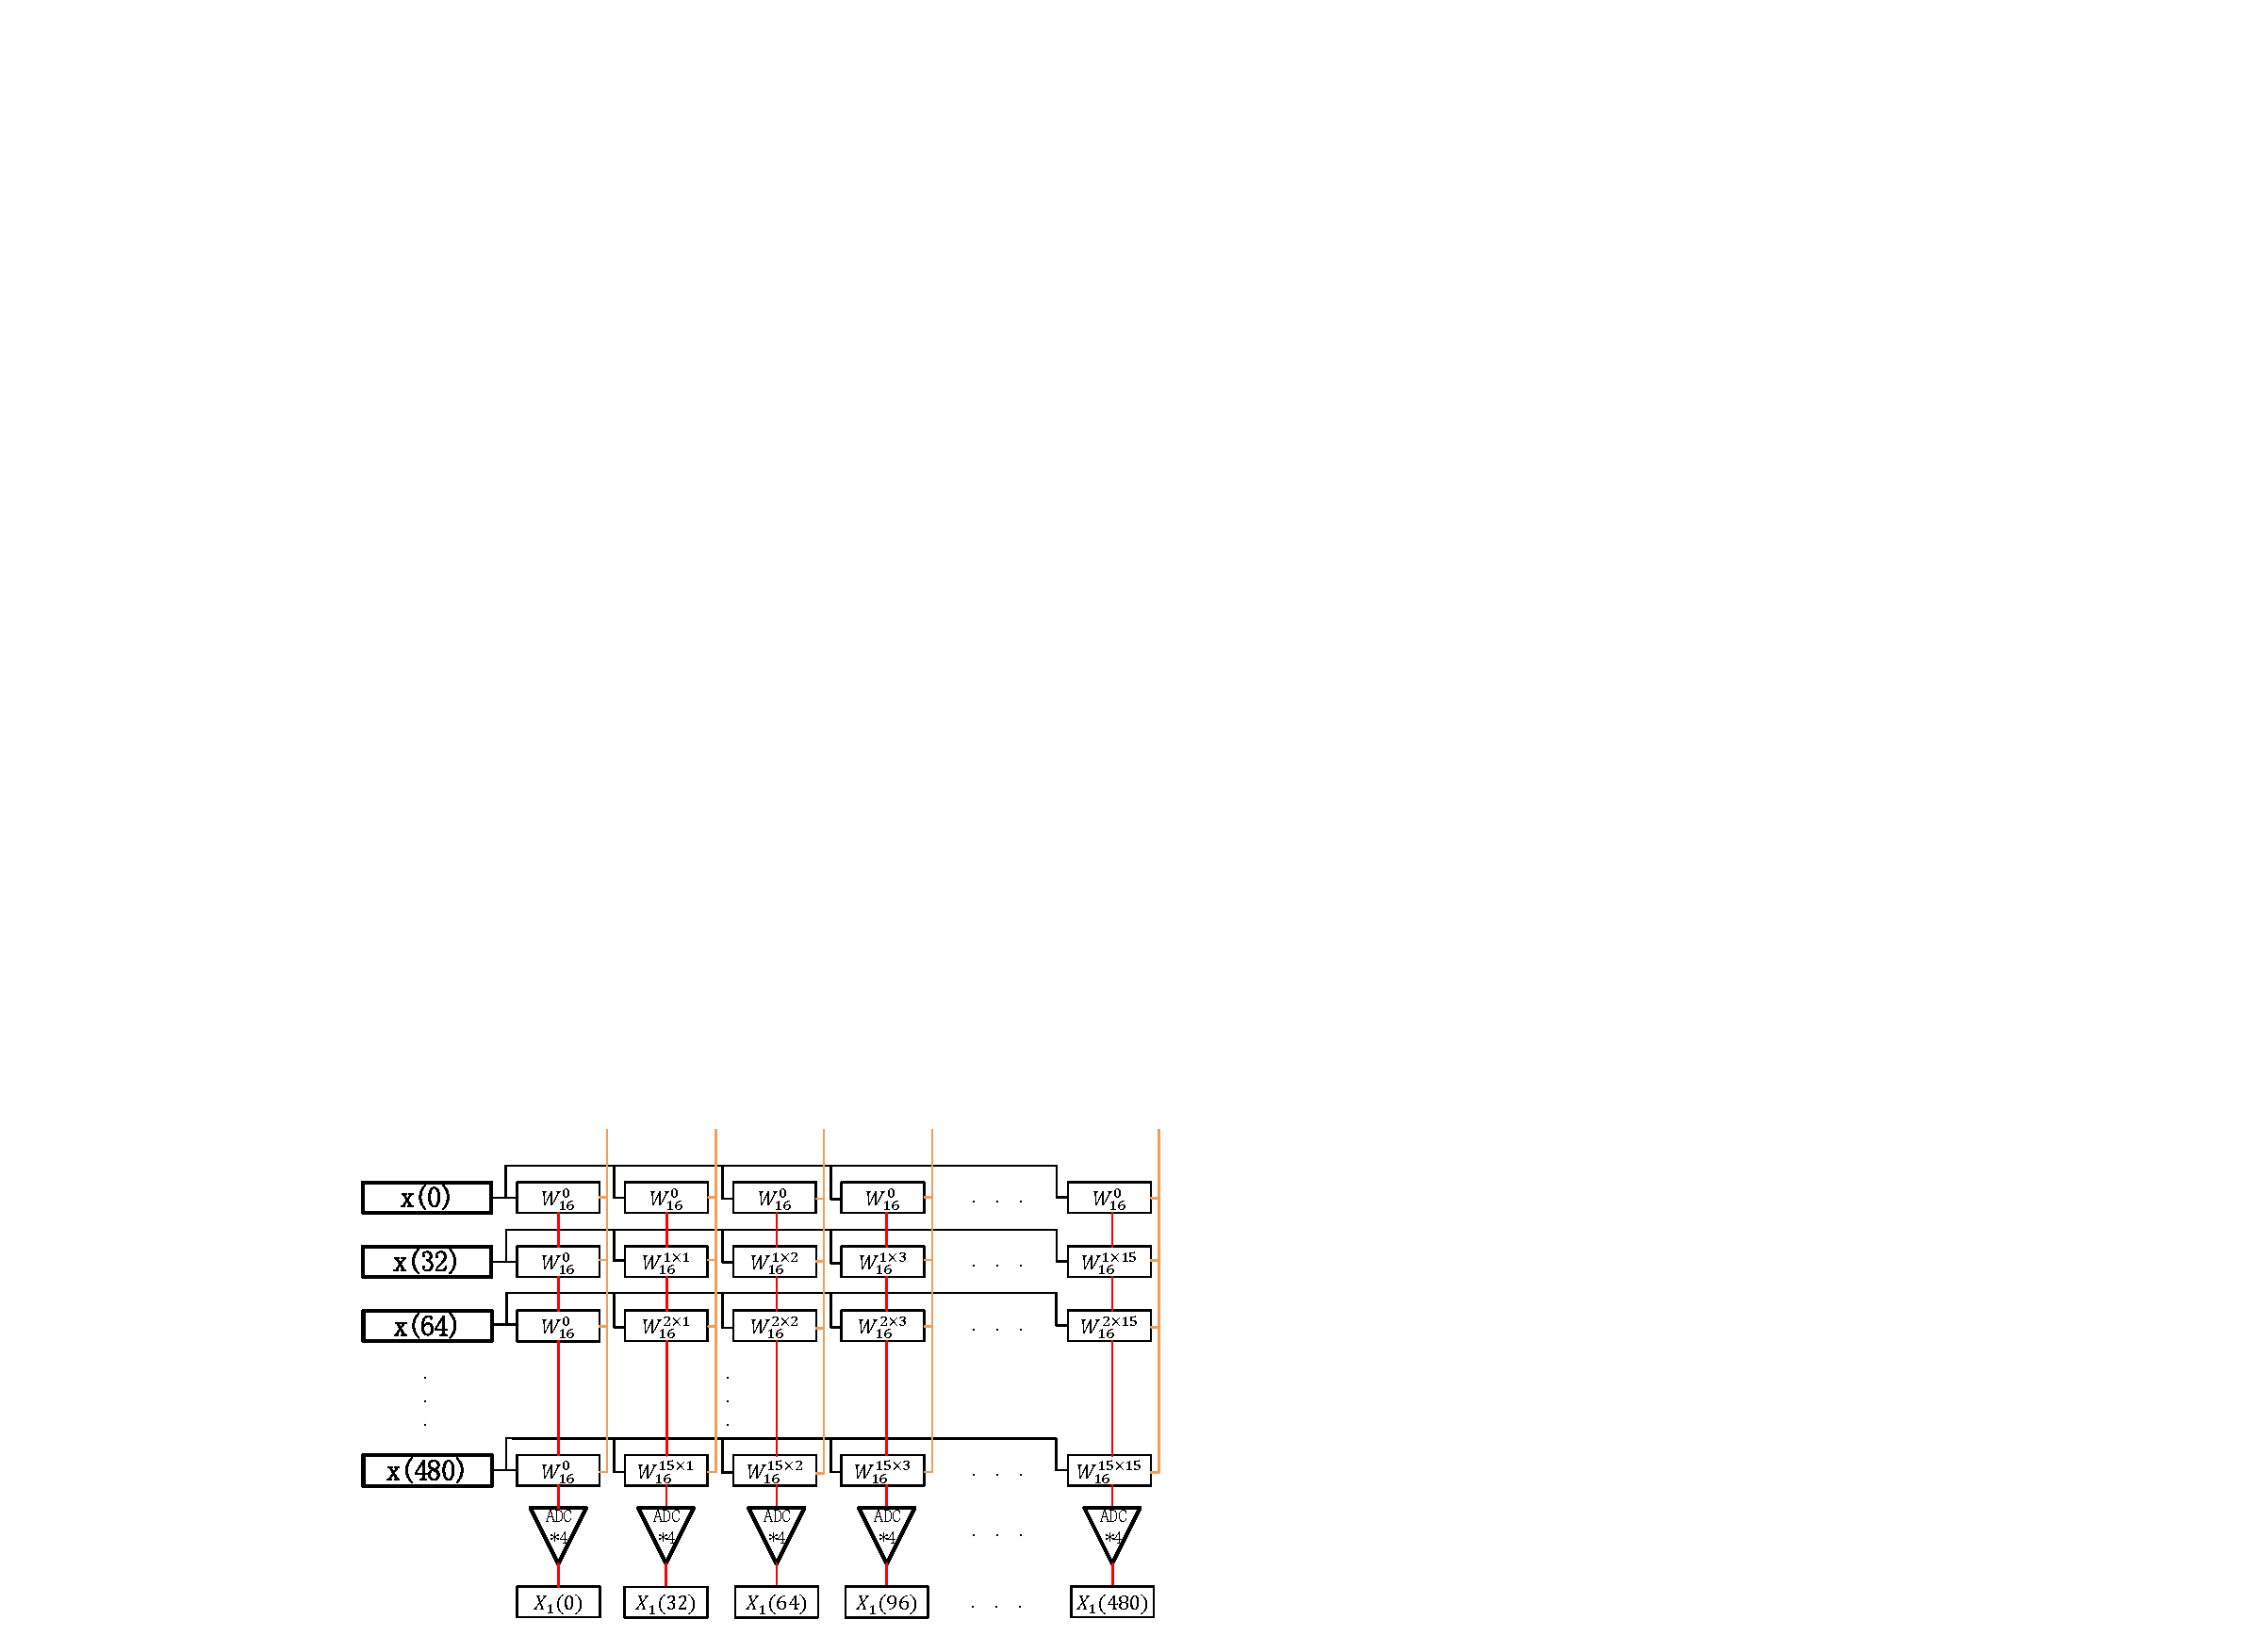
\includegraphics[scale=0.6]{figures/figure3}
\caption{The Unit Computation Core of Design}
\end{figure}


\subsection{Dataflow of Design}
In the second section, we briefly introduce the principle of mixed radix FFT. When using mixed radix, we need to pay attention to the order of data. For the butterfly operation of radix-2, we choose according to the parity of the input data order. While for the mixed radix, the data selection is more complex, so the concept of data flow is proposed here.

For example, when a 512 points FFT decomposed into 16 * 16 * 2 stages, we should generate a complex data flow. According to the formula (7)- (8), we can get the order of data entering the computation array in the first stage FFT16  and the second stage FFT 16, which is shown in fig.4 and fig.5

As shown in Figure 4, we select one data every 32 out of 512 data, so we can get 32 groups of input signal array and each group has 16 input data, just like the red dotted box in the figure. This 16 data get into the computing in memory array parallelly, and we will get 16 parallel output results. 32 groups of data repeated get into the computation core  will finish the first stage of FFT16.
\begin{figure}[h]
\centering
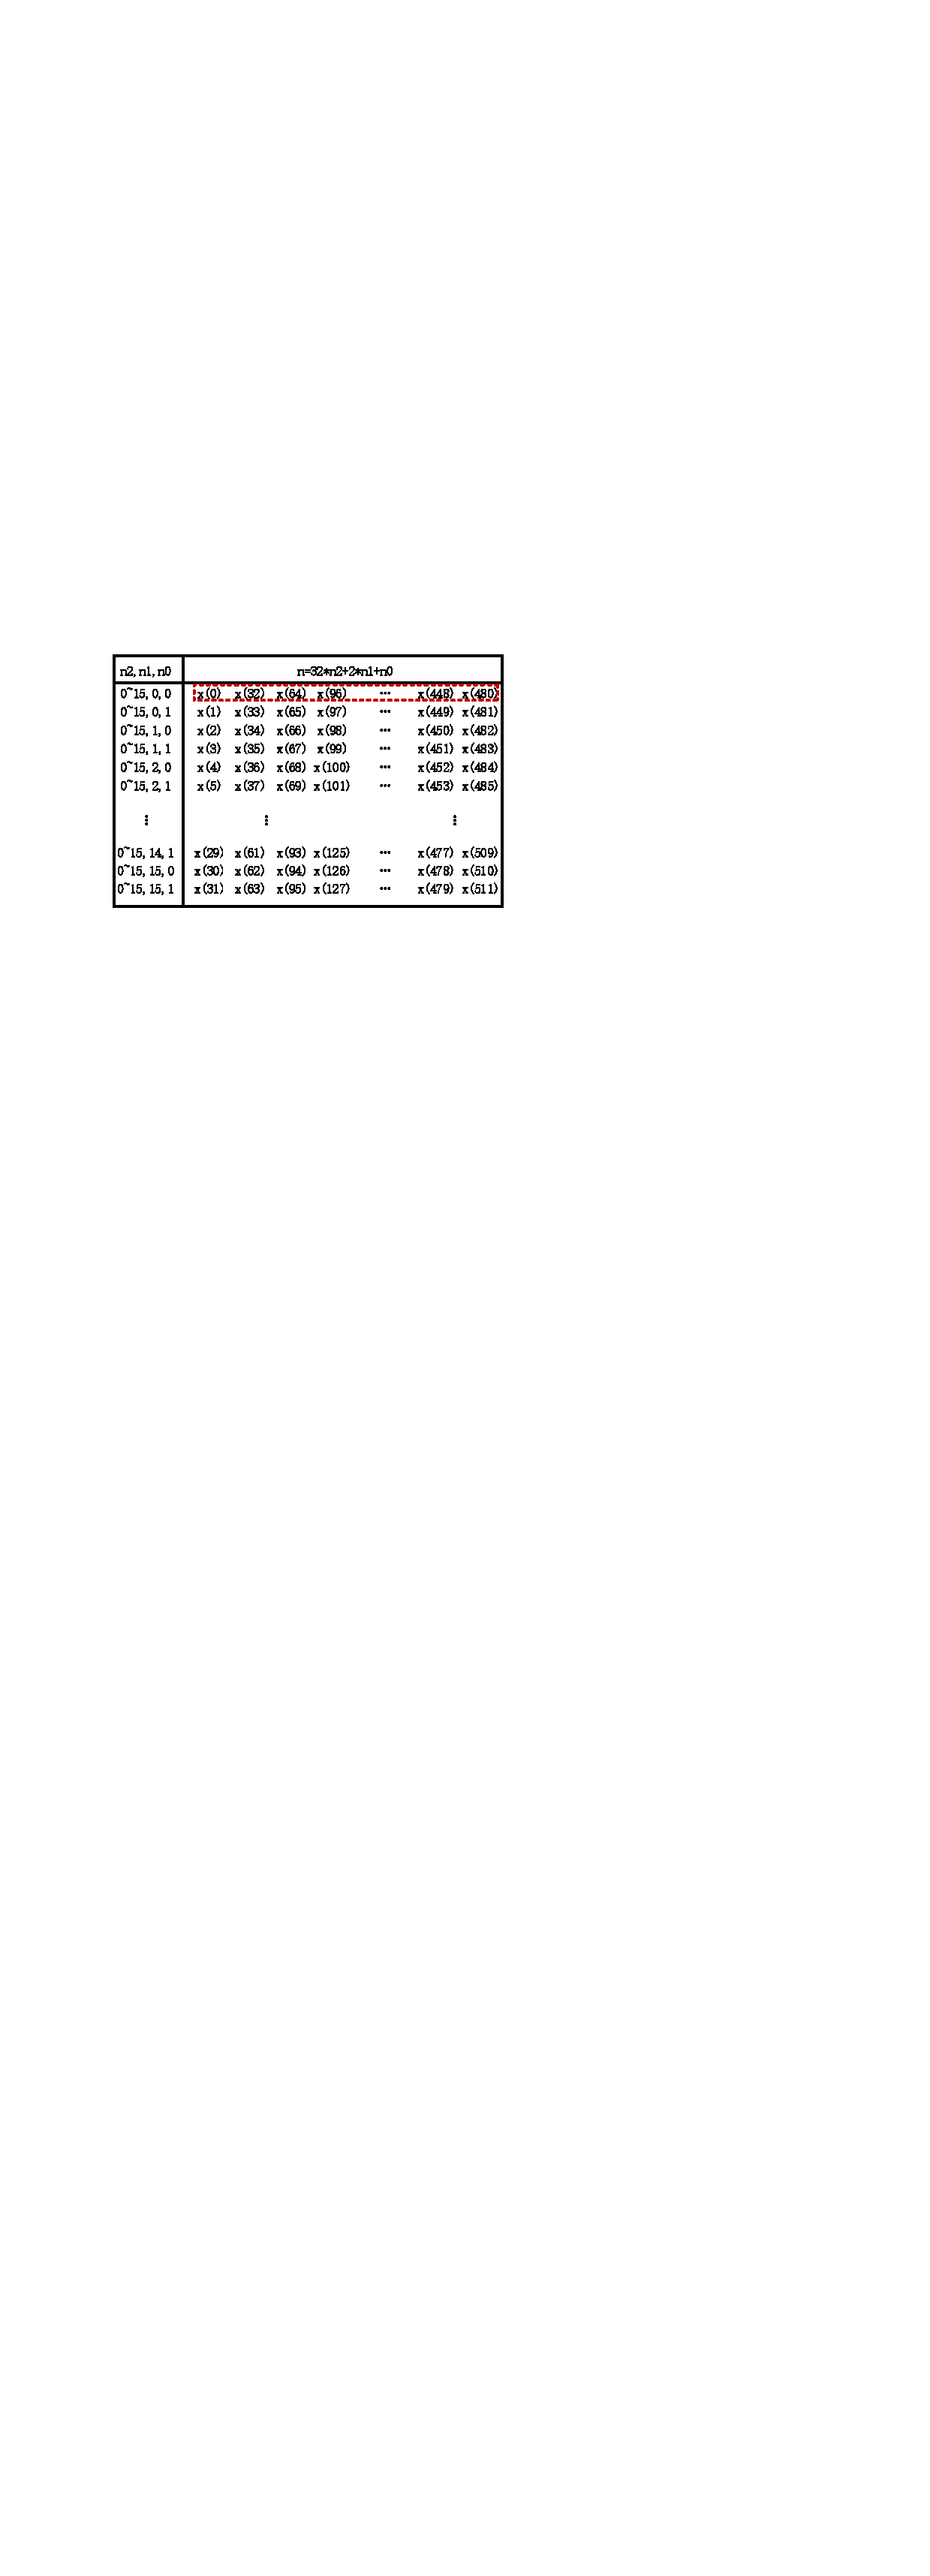
\includegraphics[scale=1]{figures/figure4.pdf}
\caption{The Order of First FFT16 Stage }
\end{figure}

On the basis of the first level calculation results, the input data of the second FFT16 stage is selected one data of every two, as shown in the red dotted box in fig.5. Similarly, we will get 32 groups of 16 input data sequences. After all the groups of data finish their computation, we will get the second stage results.It can be seen from the data of different address required by the first and second stages that such data flow generation requires a flexible controller to generate different data addresses, so that the computation results of each level can be correct.
\begin{figure}[h]
\centering

\includegraphics[scale=0.9]{figures/figure5.pdf}
\caption{The Order of Second FFT16 Stage}
\end{figure}

Figure 6 is a simple computation sequence diagram, it shows the order of data input and output in the first stage computation, while the order of the second stage is similar to that of the first, which is not shown here. It should be noted that the 8-bit input data enters the computing array in every bit, while the output data will get a 8-bit data through ADC conversion, so the input data takes longer than the output.

\begin{figure}[h]
\centering
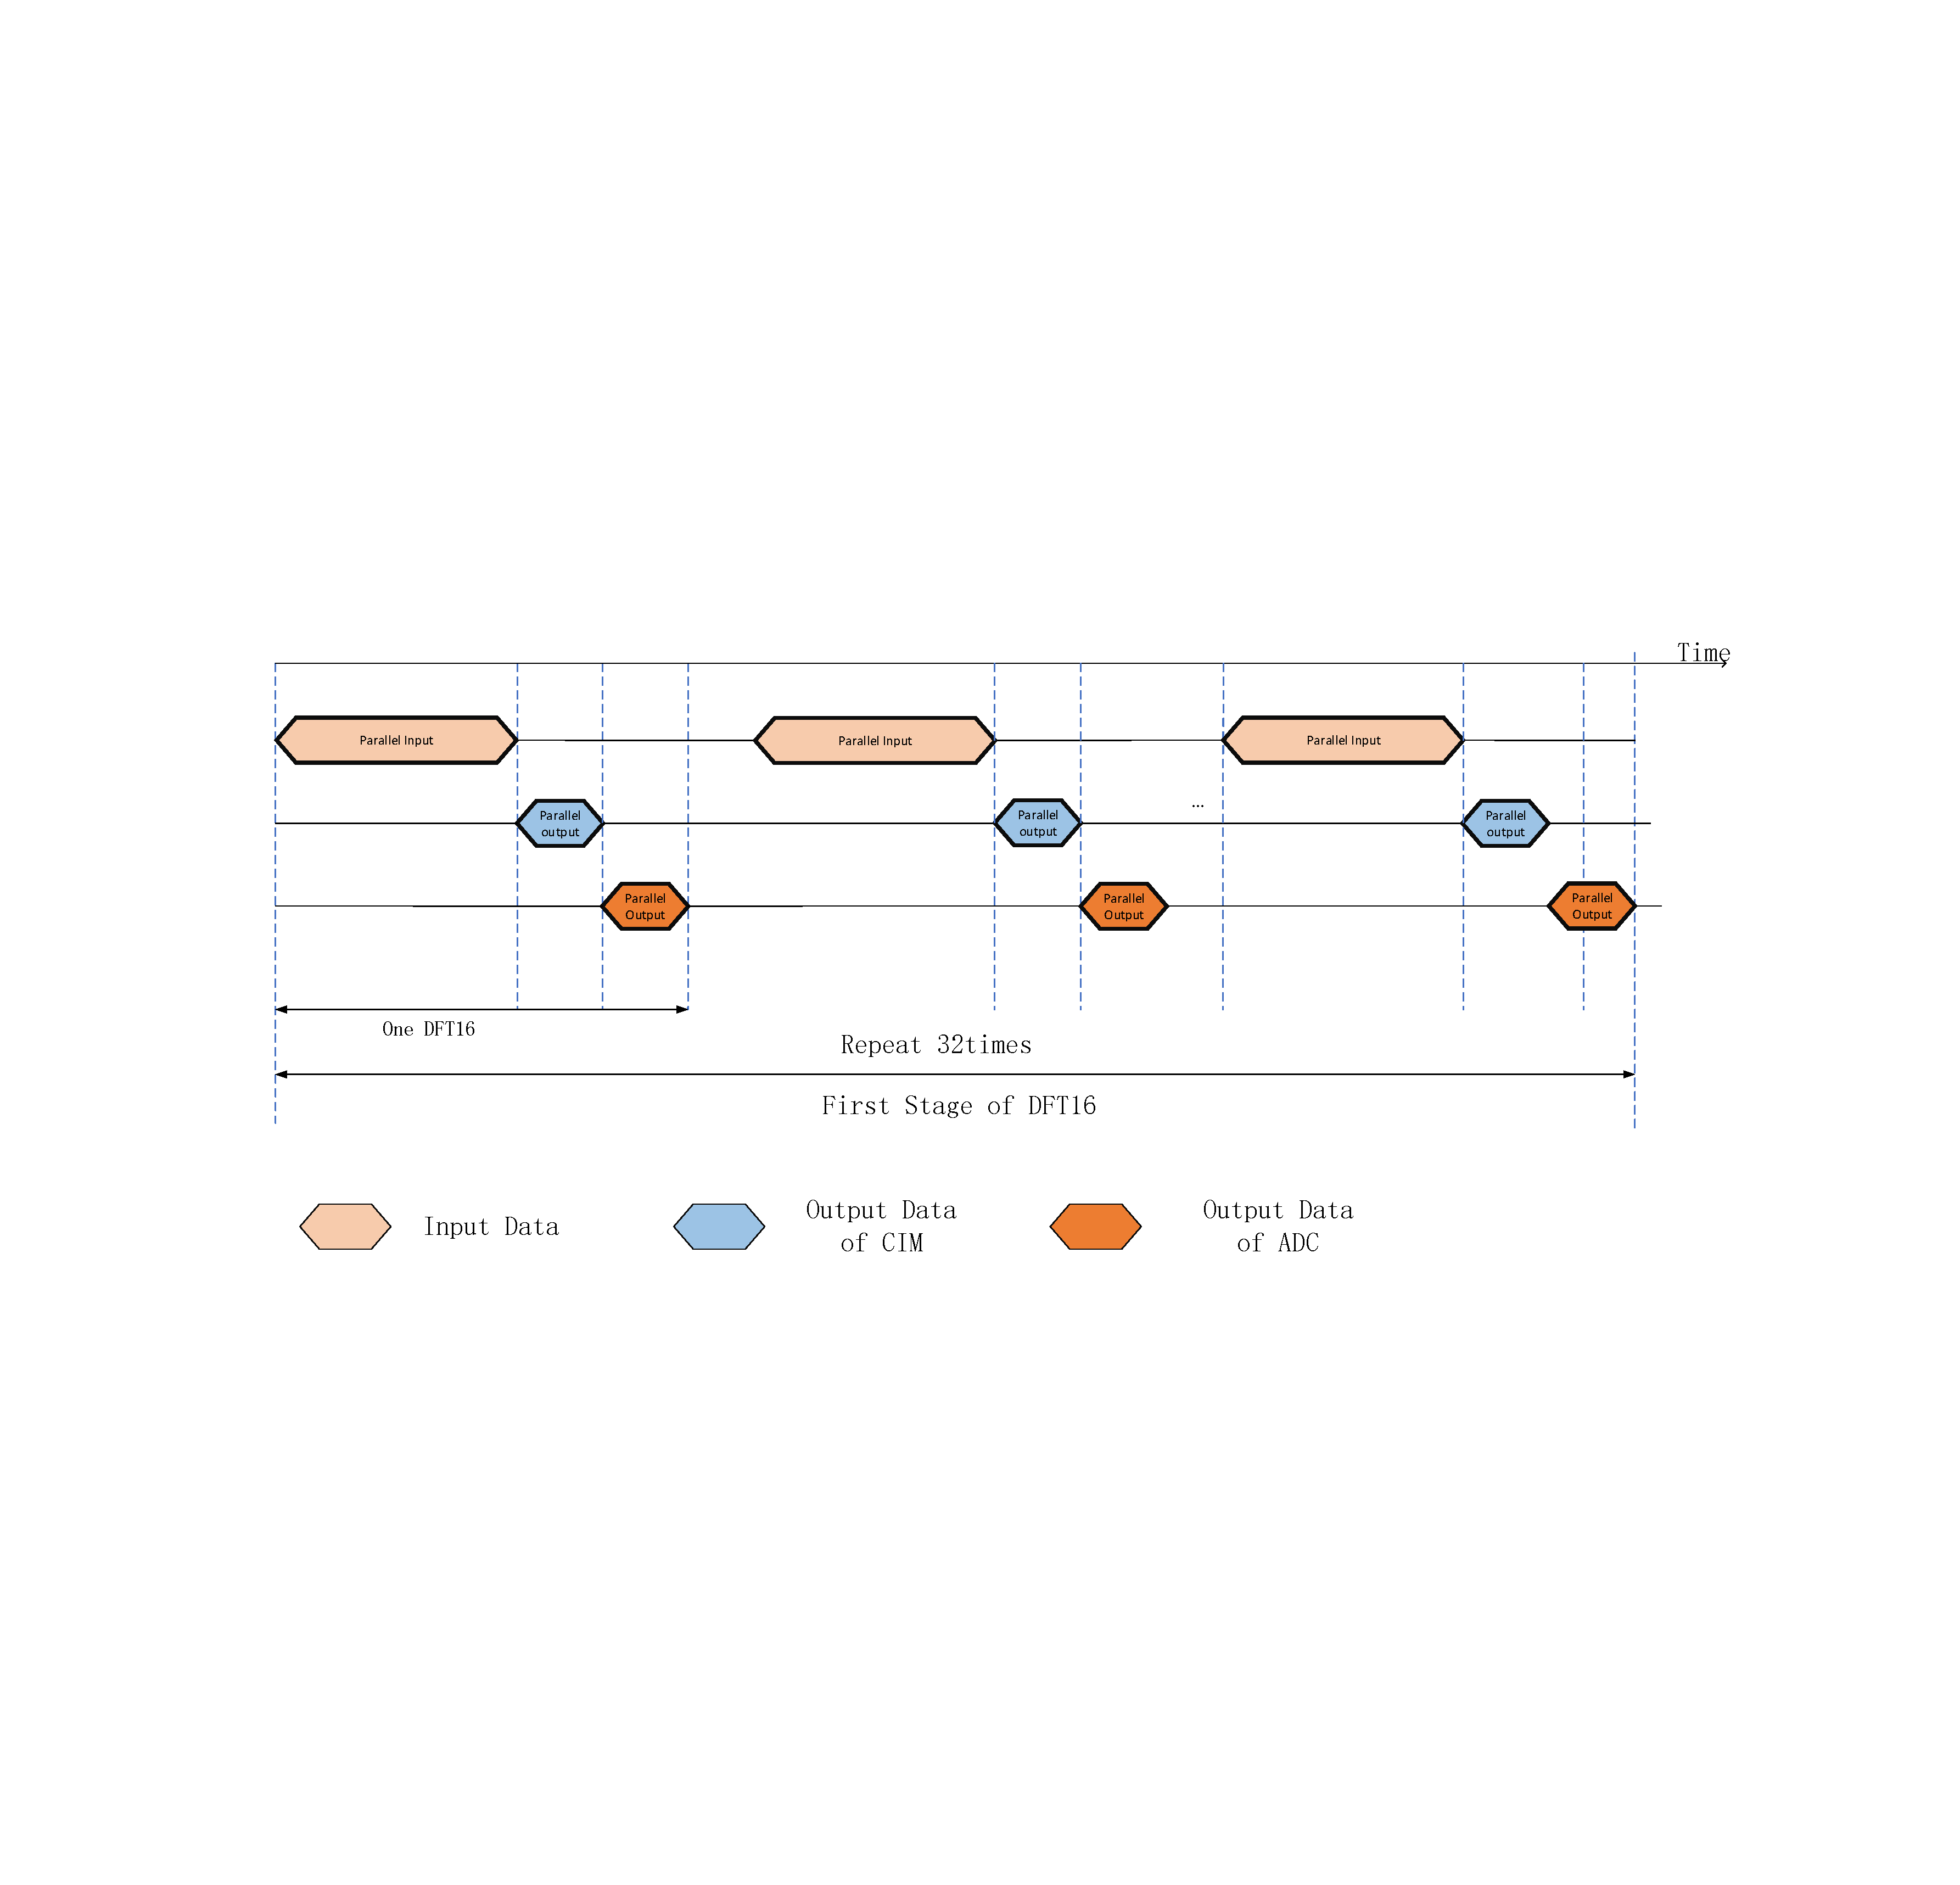
\includegraphics[scale=0.2]{figures/figure6.pdf}
\caption{The Order of Second FFT16 Stage}
\end{figure}

\subsection{Parallelism of FFT module}

Since a lot of FFT unit calculation modules are used in each stage of FFT calculation, such as the FFT16 module, we naturally think of the parallelism of FFT calculation, and the in-store calculation model provides the possibility of such parallelism. As you can see in Figure 7, when different FFT16 modules are in different columns, they can be executed in parallel. In Figure 8, every 4 DFT16 modules are executed at the same time, and the DFT16 modules that are executed at the same time are marked with the same color; while in the first and second stages of the pipeline, you can see that there are 8 DFT16 modules at the same time In execution, the same is also marked with the same color. In Figure 8, we can see the timing performance of this execution method.In this calculation method, the theoretical calculation speed can reach 4 times the previous

\begin{figure}[h]
\centering
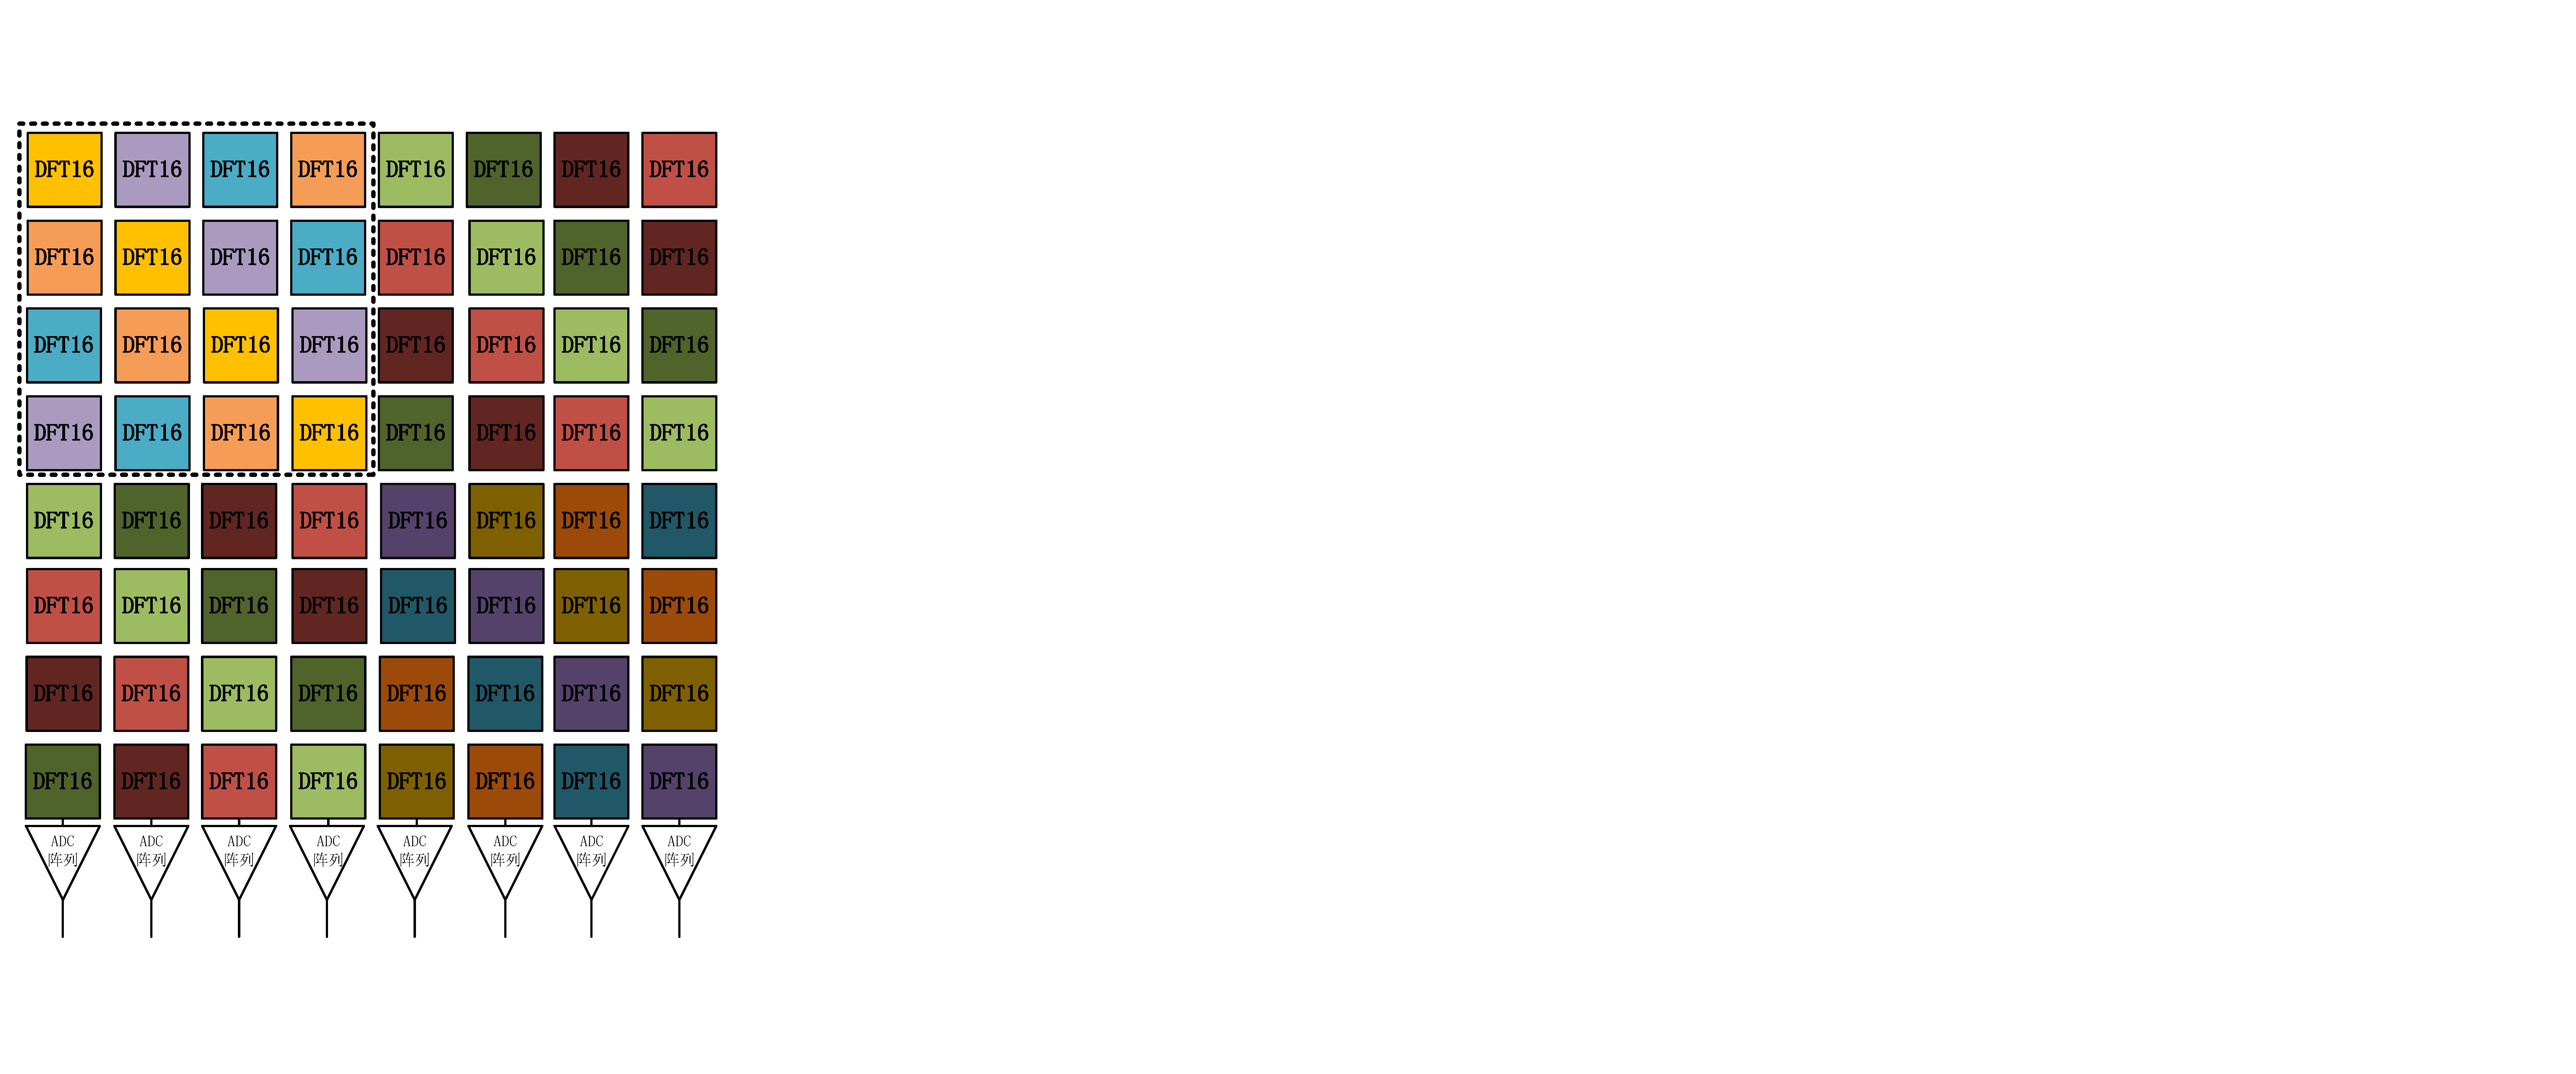
\includegraphics[scale=0.2]{figures/figure8.pdf}
\caption{The Order of Second FFT16 Stage}
\end{figure}

\begin{figure}[h]
\centering
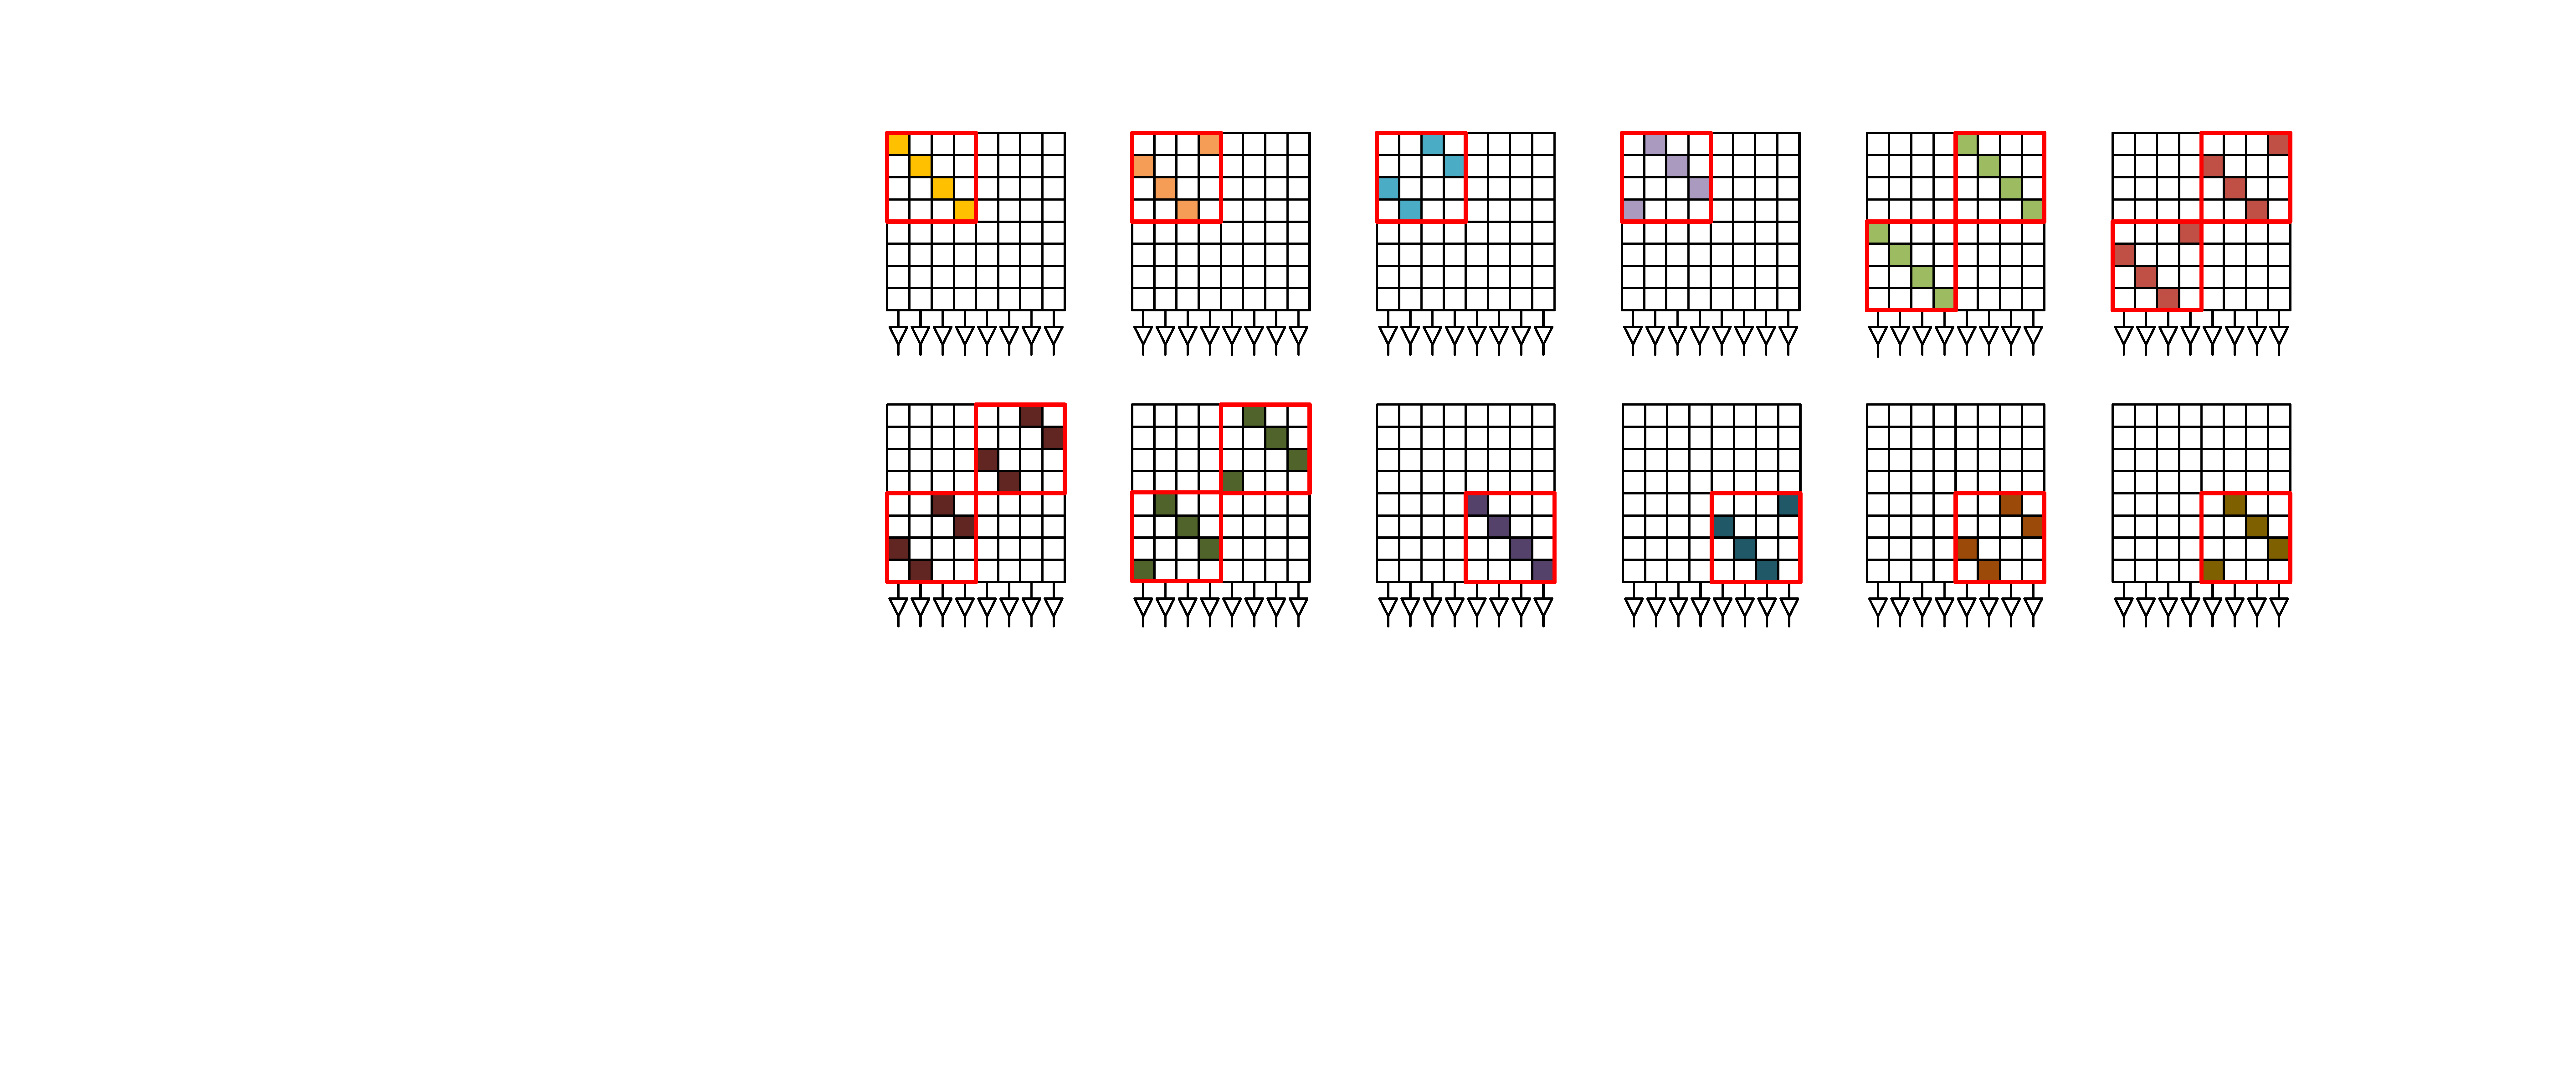
\includegraphics[scale=0.2]{figures/figure9.pdf}
\caption{The Order of Second FFT16 Stage}
\end{figure}


\subsection{Module multiplexing FFT}
Through the analysis of formulas (7)(8)(9), we can know that the twiddle factor matrix for each multiplication in the same level is the same, so in the overall calculation, it is not necessary to set all Only one or several identical matrices need to be set for the rotation factor matrix, and the overall calculation task can be completed by multiplexing these rotation factor matrices. This method is very friendly to the in-memory calculation unit, because the overall calculation can be completed by setting fewer in-memory calculation units, which greatly reduces the number of in-memory units.

\section{Experiment Result}
In this design, we use hardware description language(HDL) to model the DFT unit computing core at the behavior level, and complete the design of the whole system module, storage module and address generation module \cite{3}. Then we complete the whole experiment through functional simulation. Firstly, we use MATLAB to generate the rotation factor values of FFT with different points, and import them into the rotation factor storage file. Then, on the simulation platform, the different rotation factor data are read into the corresponding memory computing unit. At the same time, the original signal data are sent to the memory module, so we complete the initialization process of the whole system. Then, in the test platform, the address generation module generates the corresponding memory address, generates the data flow, and the data flow enters the computing in memory array according to the pre-designed way to complete the FFT calculation of each stage.

Table I shows a performance summary and comparison with previous works.


\begin{figure}[h]
\centering
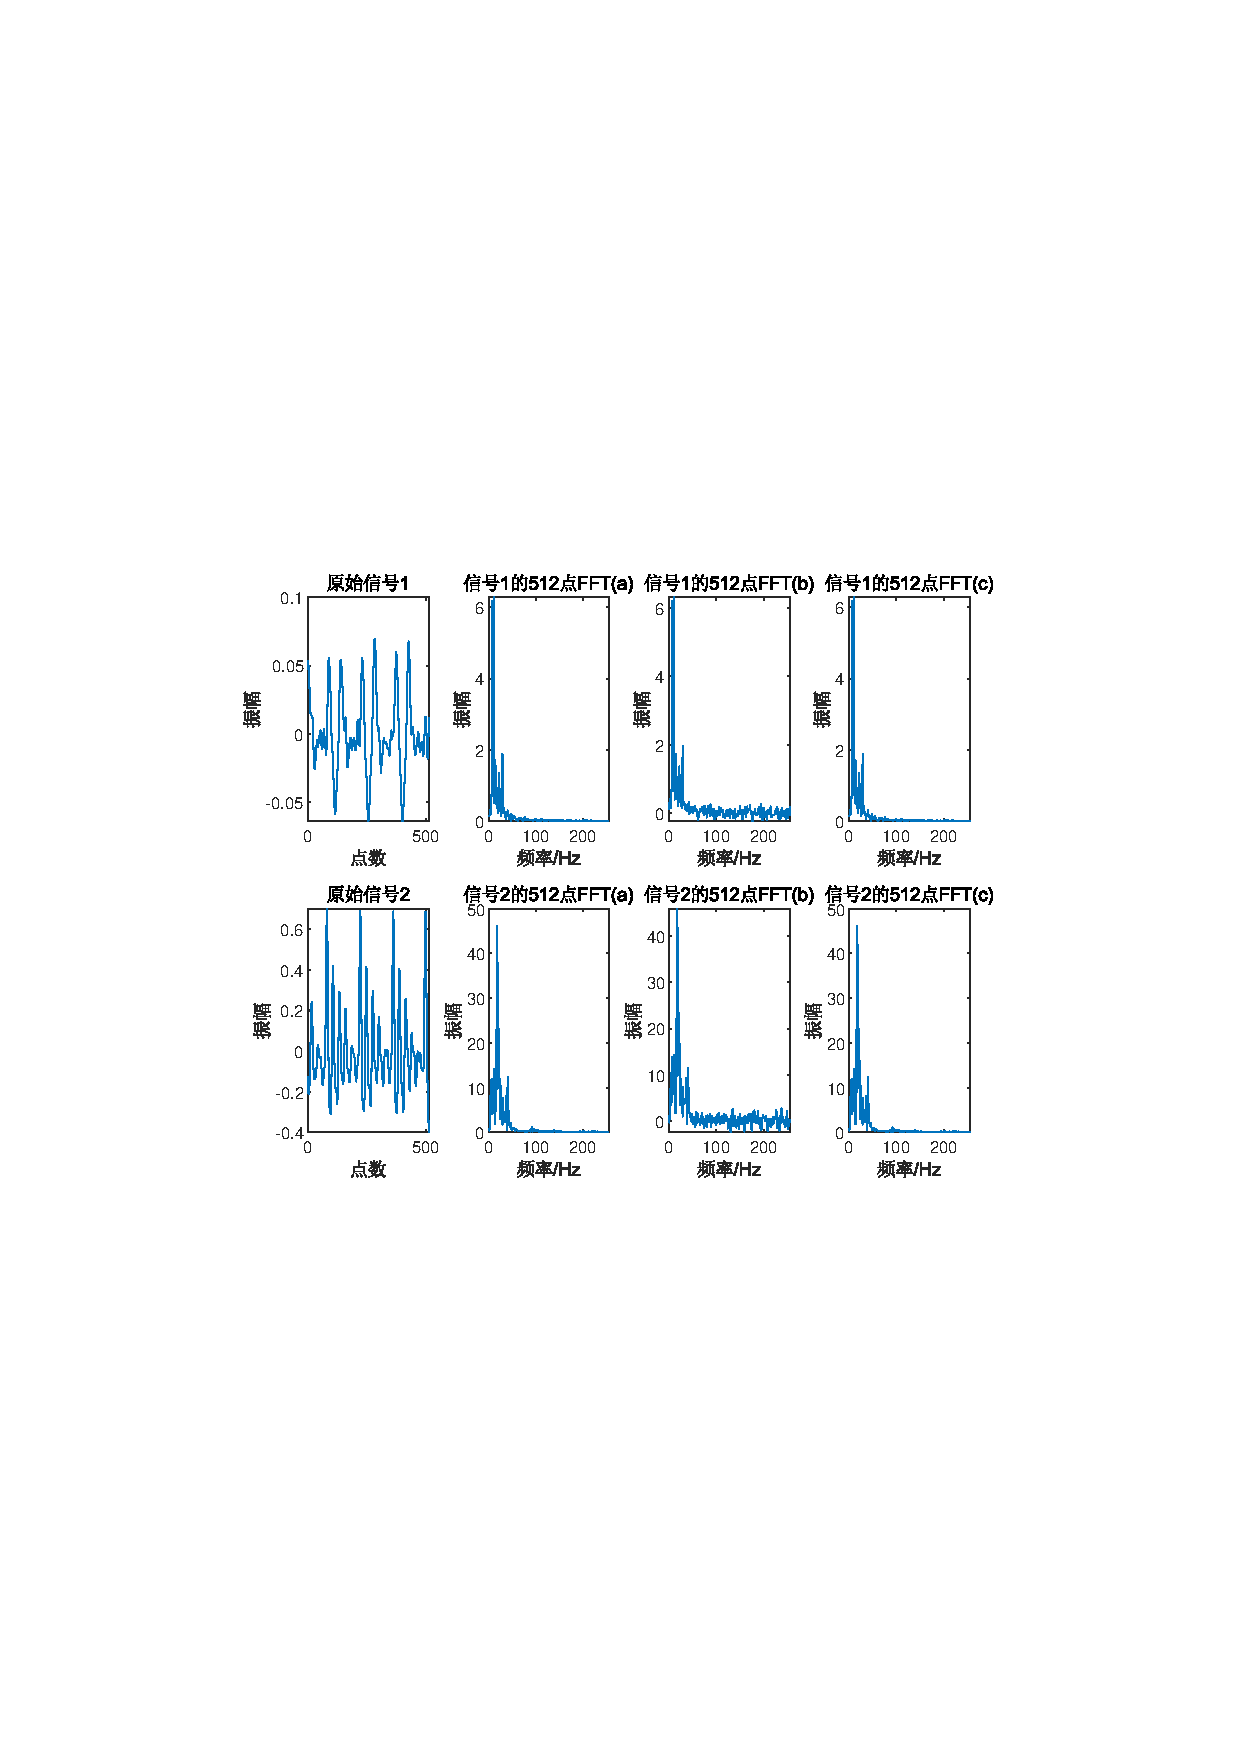
\includegraphics[scale=0.7]{figures/figure7.pdf}
\caption{Results of FFT analysis}
\end{figure}

\section{Conclution}
This paper first expounds the possibility of combining CIM with FFT, and then analyzes the specific problems that may arise in the design process, that is, the number of FFT points is too large to be computed directly in CIM array. Then, a mixed radix decomposition method is proposed to decompose the large-scale DFT matrix into several small-scale DFT matrices, which successfully solves the above problems. In order to complete the design, the DFT computation unit and the data flow control unit, namely the address generation module, are implemented at the same time\cite{4}. Finally, the overall design achieves good \cite{5} computing \cite{6} performance and power \cite{7} consumption.


\begin{table}[htbp]
\centering
\caption{Comparison with Reference Works}
\label{Tab I}
    \begin{tabular}{cccccc}
        \hline
        Specification &Proposed &[1](F) &[2](P) &[2]      &[3] \\
        \hline
        FFT Size(N)   &512      &1024   &1024   &1024     &4096   \\
        Technology    &45nm     &65nm   &65nm   &65nm     &65nm   \\
        Vdd           &1V       &0.45V  &0.45V  &0.6V     &1.2V   \\
        Word-length   &8-bit    &12-bit &12-bit &32-bit*  &14-bit  \\
        Power(mW)     &21.66    &12     &123    &60.3     &68.6    \\
        \hline
    \end{tabular}
\end{table}


% Can use something like this to put references on a page
% by themselves when using endfloat and the captionsoff option.
\ifCLASSOPTIONcaptionsoff
  \newpage
\fi

\bibliographystyle{IEEEtran}
\bibliography{reference}


\end{document}


